\documentclass{beamer}

\mode<presentation> {
	\usetheme{Antibes}
	\setbeamertemplate{footline}[page number]	
	\setbeamertemplate{navigation symbols}{}
	\setbeamertemplate{items}[square]
}

\usepackage{graphicx}
\usepackage{booktabs}
\usepackage{hyperref}

\newcommand{\link}[2]{\href{#1}{\textit{\color{blue}{#2}}}}%


\title[DragonFly]{Project DragonFly: Vehicle Surveillance System}
\institute[GCEK-CSE]{Department of Computer Science and Engineering \\Government College of Engineering Kannur}
\author[Group 3]{
	{\small \textit{Guided by:}} Dr. Rafeeque P.C \\
	\medskip
	{\small \textbf{\textit{Group 3}}} \\
	Abhinand C \\ Edwin Jose George \\ Lavanya E.V \\ Shilpa Suresh
}
\date{\today}

\begin{document}
	
	%---------------------------------------------------------------------------
	% METADATA -----------------------------------------------------------------
	%---------------------------------------------------------------------------

	\begin{frame}
	\titlepage
	\end{frame}

	\begin{frame}{Table of Contents}
	\tableofcontents
	\end{frame}


	%---------------------------------------------------------------------------
	% INTRODUCTION -------------------------------------------------------------
	%---------------------------------------------------------------------------

	\section{Introduction}
	\subsection{Objective}
	\begin{frame}{Objective}
		
		Policing agencies have setup vast networks of distributed surveillance cameras along major routes. The sheer amount of data generated is overwhelming for manual analysis, to trace routes of rouge vehicles.\\~\\
				
		DragonFly is an AI based project that aims to resolve this particular issue. 
	\end{frame}
	
	\subsection{Proposed System}
	\begin{frame}{Steps}
		\begin{itemize}
			\item The user provides the system with vehicle descriptions such as color, make,
			model, location, time-period etc. 
			\item The system finds corresponding match by making
use of various AI techniques. 
			\item The system tries to re-identify the said vehicle across multiple camera locations.
			\item The system finds the path followed by the said vehicle
along with the detected frame at each camera points.
		\end{itemize}
	\end{frame}
	
	\begin{frame}{Architecture Design}
		\begin{center}
			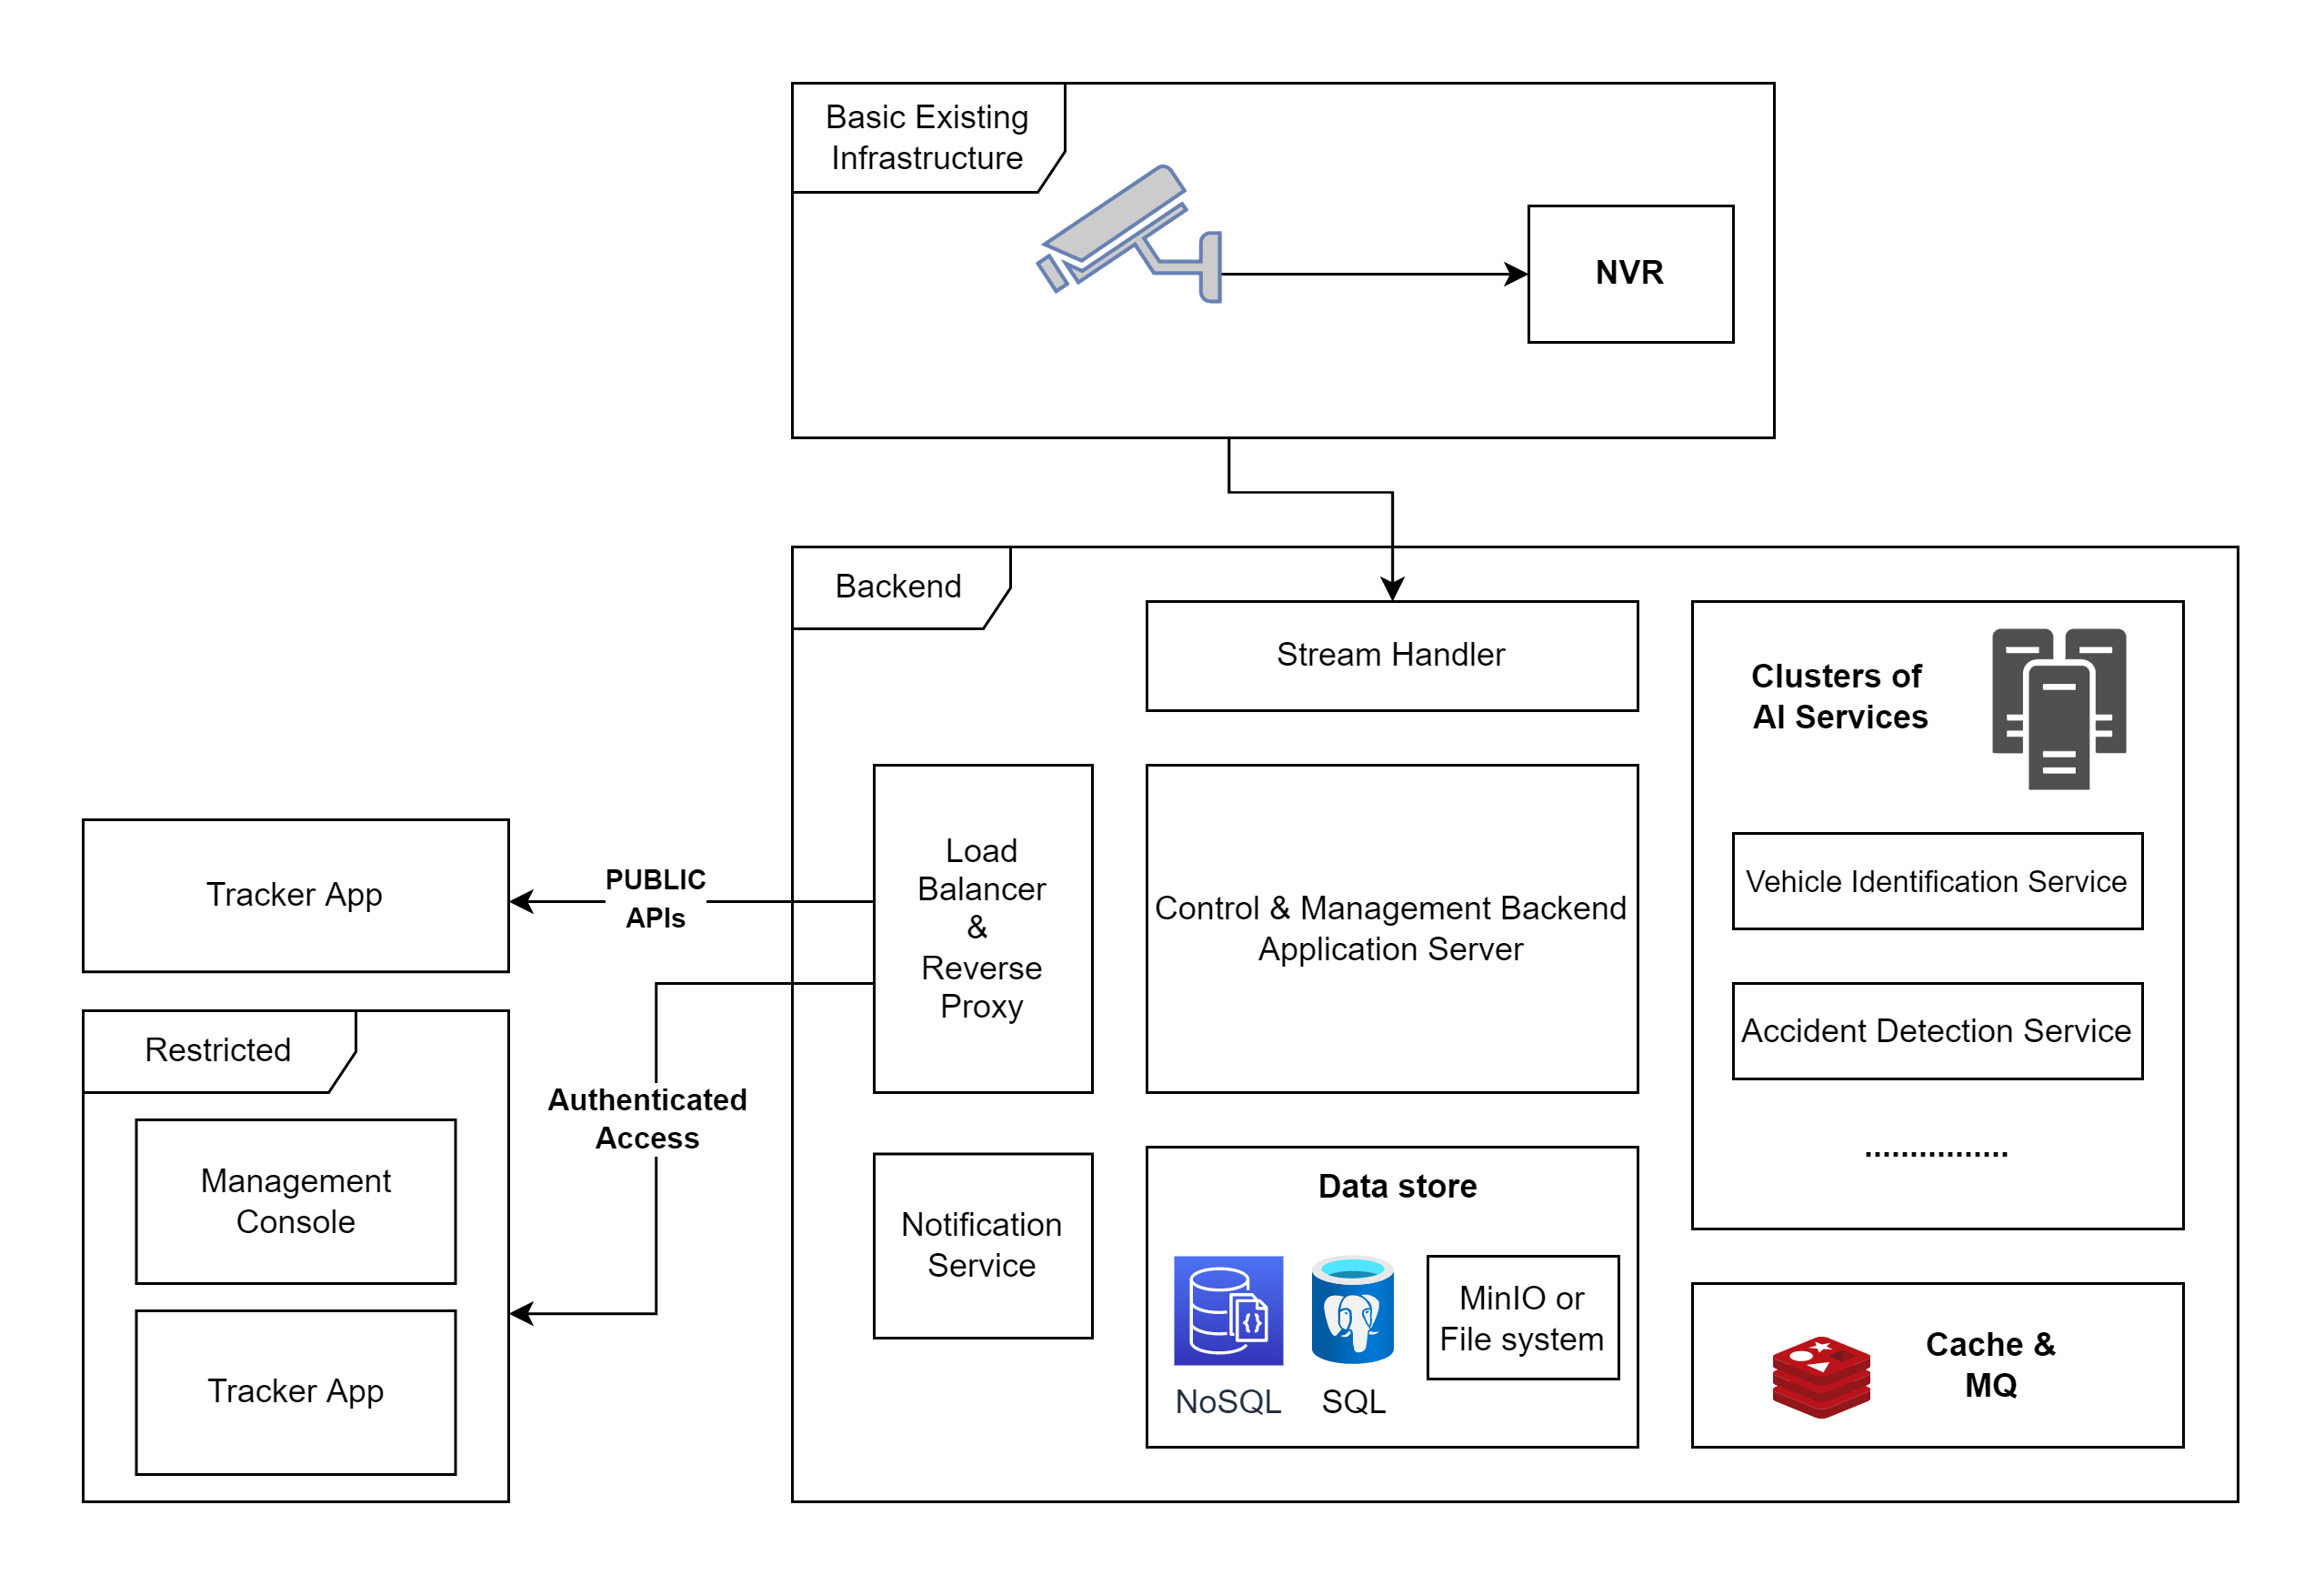
\includegraphics[width=\linewidth]{res/architecture_high_level}
		\end{center}
	\end{frame}

	\begin{frame}{Pipeline1}
		\begin{center}
			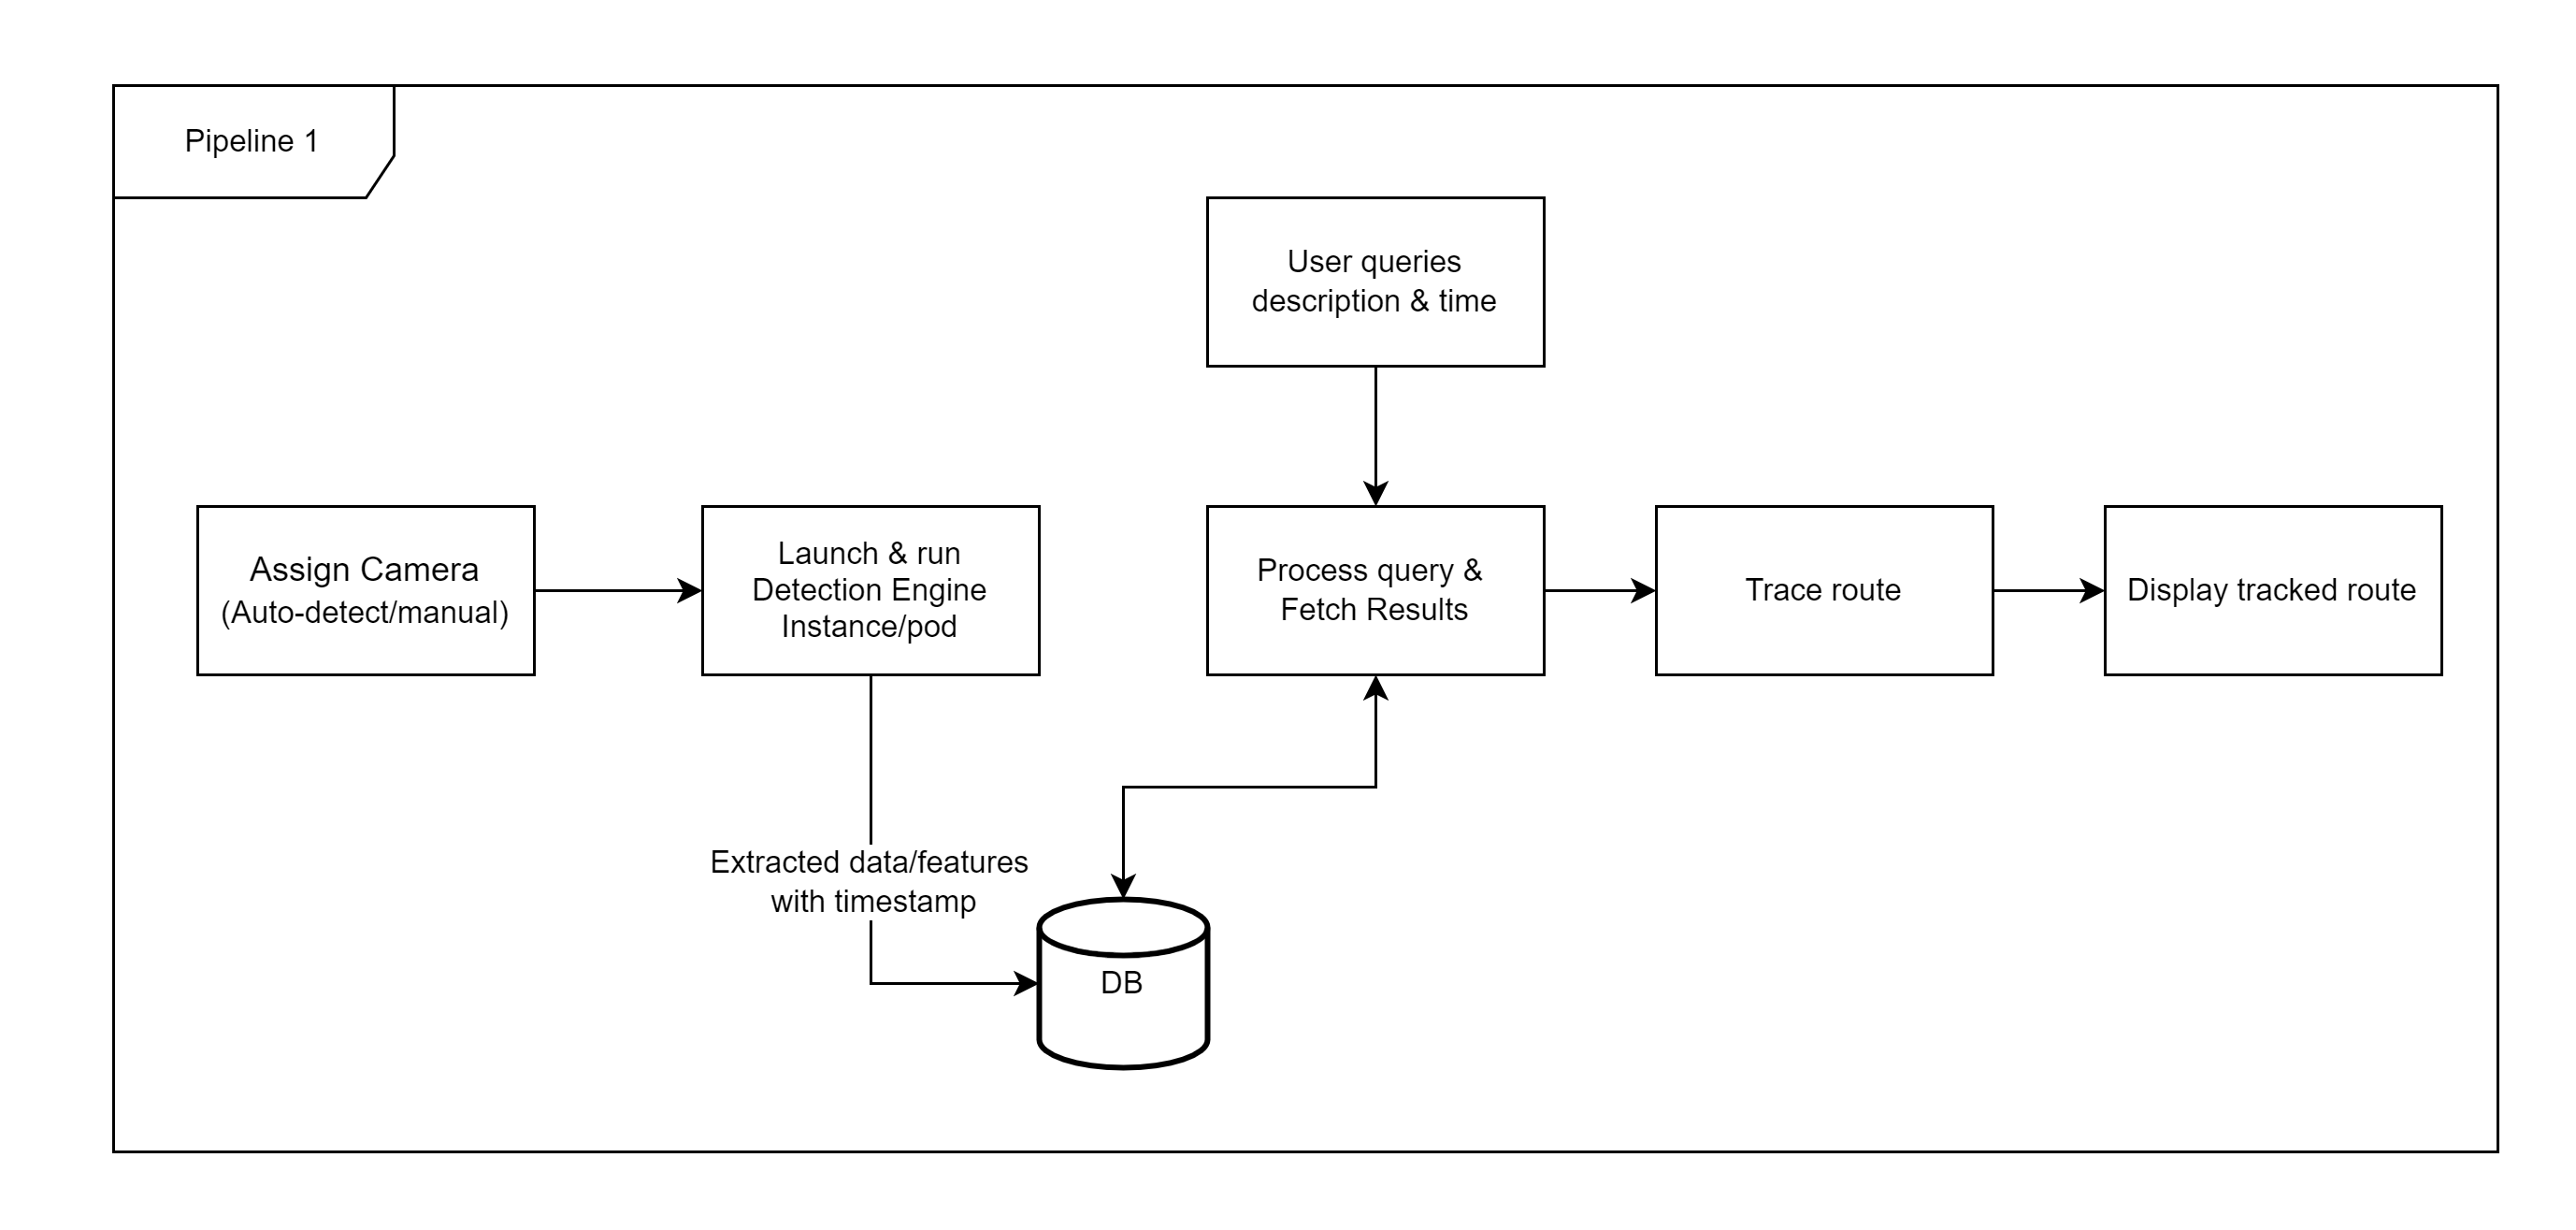
\includegraphics[width=\linewidth]{res/pipeline1}
		\end{center}
	\end{frame}

	\begin{frame}{Pipeline2}
		\begin{center}
			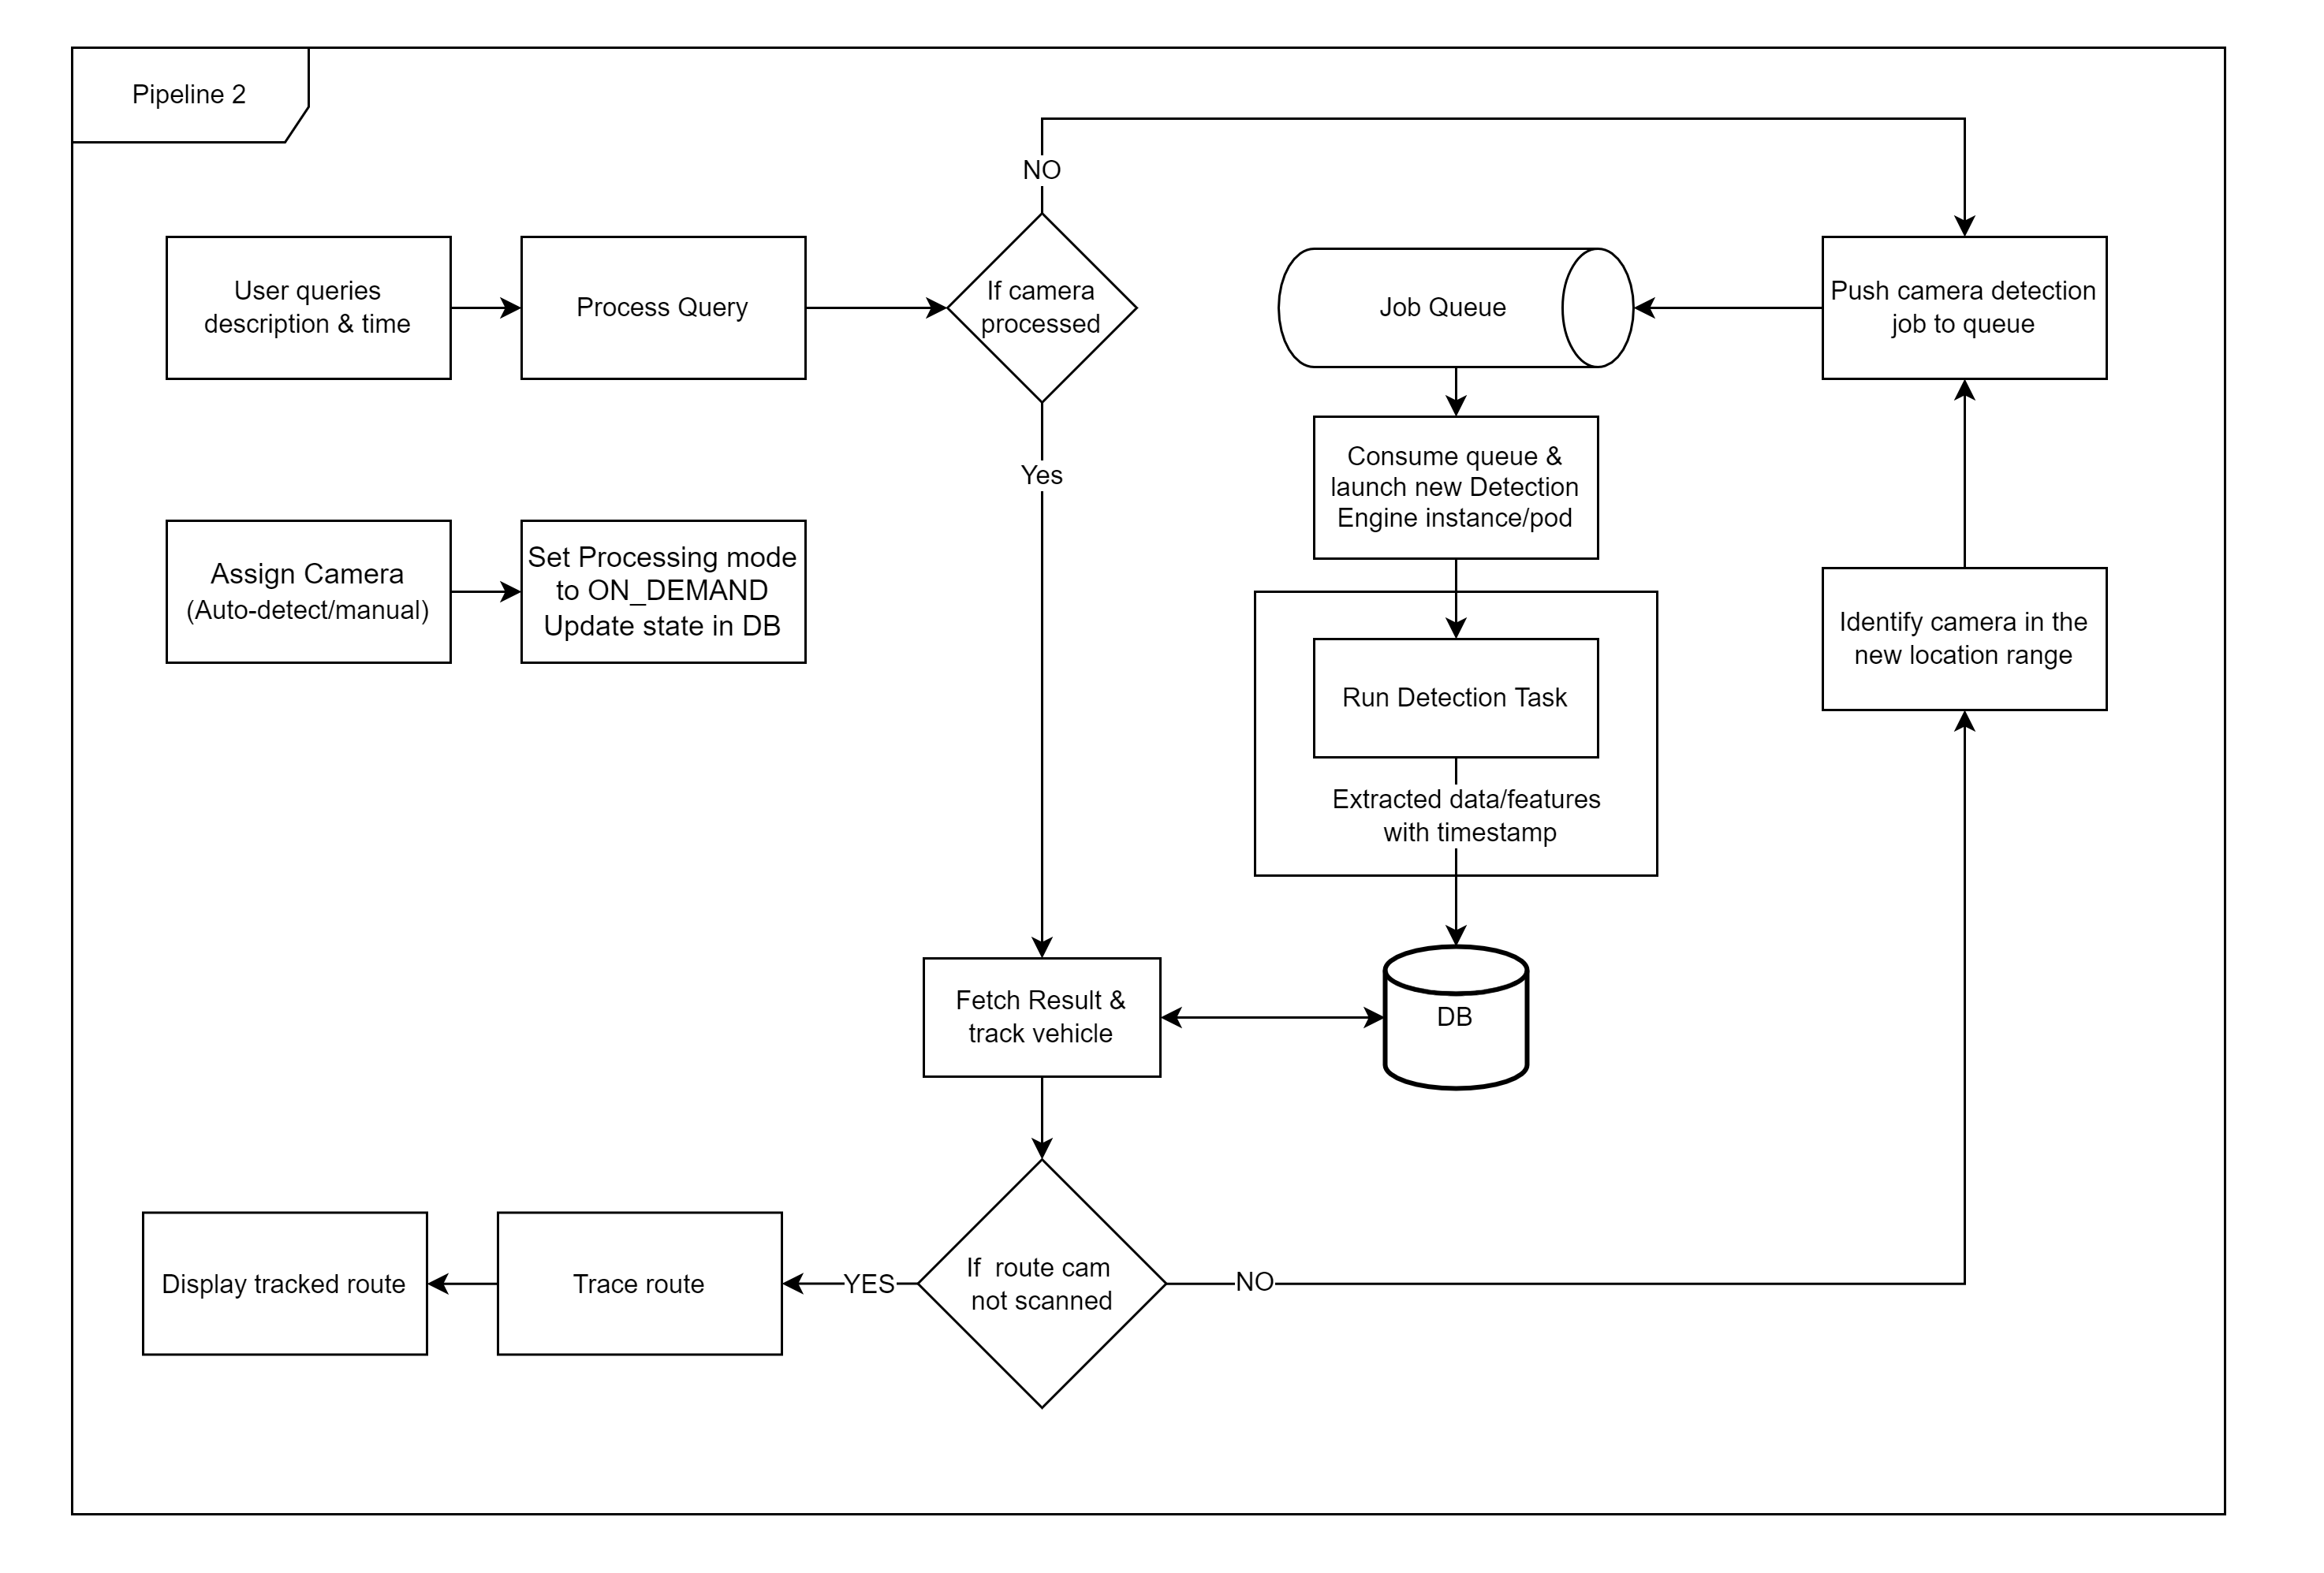
\includegraphics[width=\linewidth]{res/pipeline2}
		\end{center}
	\end{frame}


	%---------------------------------------------------------------------------
	% WORKS DONE SO FAR --------------------------------------------------------
	%---------------------------------------------------------------------------

	\section{Works done so far}
	\subsection{AI model}
	\begin{frame}{Experimented with Classical Object detection methods}
		\begin{itemize}
			\item K-Means algorithm used for color extraction
				\link{https://github.com/Project-Dragon-Fly/tutorial-trials/blob/tutorial\_testing/Color\%20detection.ipynb}{notebook}
			
			\item Using OpenCV to detect object  
				\link{https://github.com/Project-Dragon-Fly/tutorial-trials/blob/tutorial\_testing/OpenCV-image-difference.ipynb}{notebook} $|$ 
				\link{https://drive.google.com/file/d/1-2EAoUBxMzfnMO3tVJFJ0qvGnXMFp4zL/view}{video}
			
			\item Harr algorithm to detect Bus and Car
				\link{https://github.com/Project-Dragon-Fly/tutorial-trials/blob/tutorial\_testing/OpenCV\%20-\%20Haar\%20algo.ipynb}{notebook} $|$
				\link{https://drive.google.com/file/d/1XYbVf6I2ZJSSdO2SsZECK9rNoYQwROM9/view}{video}
		\end{itemize}
		\begin{small}
			Video are generated using the code mentioned in this \link{https://github.com/Project-Dragon-Fly/tutorial-trials/blob/tutorial\_testing/Detection\_video\_generator.ipynb}{notebook}
		\end{small}
	\end{frame}

	\begin{frame}{Exploring various AI methods}
	\begin{itemize}
		\item Several YouTube tutorials and web articles are referenced to get understanding of AI methods and its evolution, which are summarized in this \link{https://docs.google.com/presentation/d/1ugCdqNADQ1QNd91lMP4BmbFBKYhkMoDrN2yIf\_t7SkI/edit?usp=sharing}{google slides}.
		
		\item Tensorflow provided this \link{https://github.com/Project-Dragon-Fly/tutorial-trials/blob/tutorial\_testing/object\_detection\_tensorflow\_tutorial.ipynb}{notebook} showing the usage of mobile-ssd/f-rcnn to detect general objects.
		
		\item Followed through the beginners tutorial provided by Tensorflow Team, saved at \link{https://github.com/Project-Dragon-Fly/tutorial-trials/tree/tutorial\_testing/YouTube\%20Tutorial\%20-\%20TensorFlow}{github}.
		\begin{itemize}
			\item Emphasis on working of CNN
			\item Got at glance at intermediate layer output of horse-human classifier. Output saved at  \link{https://github.com/Project-Dragon-Fly/tutorial-trials/blob/tutorial\_testing/YouTube\%20Tutorial\%20-\%20TensorFlow/Tutorial\%204\%20-\%20CNN\%20on\%20complex\%20images.ipynb}{notebook}
		\end{itemize}
	\end{itemize}
\end{frame}

	\subsection{UI/UX}	
	\begin{frame}{Works done : UI/UX}
		User Interface updates
	\end{frame}

	\subsection{Other Updates}
	\begin{frame}{Works done : Other updates}
		Other updates
	\end{frame}

\end{document} 